\chapter{Installation and Making it Work}
Palladian depends on Java 1.6. If you are using Linux, make sure to use Sun's proprietary JDK instead of OpenJDK to avoid build problems\footnote{Open a Terminal and enter \texttt{java -version} to check the currently installed Java version. The necessary steps to change your Java version depend on your Linux distribution, for Ubuntu flavours see \url{https://help.ubuntu.com/community/Java}.}. The code base is managed using \href{http://subversion.apache.org/}{Subversion (SVN)} (see Chapter~\ref{sec:toolkitstructure}). It is build and tested automatically on every commit using \href{http://maven.apache.org/}{Apache Maven} and \href{http://jenkins-ci.org/}{Jenkins CI}. Bugs might be reported using the \href{http://www.redmine.org/}{Redmine bugtracker}. The project encoding is UTF-8. To support unavailable libraries we manage our own Maven repository using \href{http://nexus.sonatype.org/}{Sonatype Nexus}. How to use these components is explained in the next sections.

Currently each systems manages its own user base so registration is needed for each one. To start working with the toolkit you should send an E-Mail to a toolkit administrator to get access to the systems. Provide your name, the name of your advisor and the reason why you need to work with the toolkit and you will get your logins.
\section{Building Palladian using Apache Maven}
\label{sec:buildingthetoolkitusingapachemaven}
Apache \textbf{Maven needs to be installed} to build the toolkit. Instructions for how to \href{http://maven.apache.org/download.html#Installation}{install Maven} can be found in the link. There is one manual step before you can start building the toolkit. You need to add our Nexus repository to your local Maven settings. Do this by \textbf{locating or creating the settings.xml file in your local home folder:} \texttt{\%YOUR\_HOME\_FOLDER\%/.m2/settings.xml} and adding the following content, replacing both user and password as provided by the toolkit administrator:
\begin{verbatim}
<settings xmlns="http://maven.apache.org/SETTINGS/1.0.0"
  xmlns:xsi="http://www.w3.org/2001/XMLSchema-instance"
  xsi:schemaLocation="http://maven.apache.org/SETTINGS/1.0.0
                      http://maven.apache.org/xsd/settings-1.0.0.xsd">
  <servers>
    <server>
      <id>snapshots</id>
      <username>palladian</username>
      <password>wisdom</password>
      <filePermissions>664</filePermissions>
      <directoryPermissions>775</directoryPermissions>
      <configuration></configuration>
    </server>
    <server>
      <id>releases</id>
      <username>palladian</username>
      <password>wisdom</password>
      <filePermissions>664</filePermissions>
      <directoryPermissions>775</directoryPermissions>
      <configuration></configuration>
    </server>
  </servers>
</settings>
\end{verbatim}
% You need to set your username and your password in the server section. This can be obtained by sending an E-Mail to \href{mailto:klemens.muthmann@tu-dresden.de}{klemens.muthmann@tu-dresden.de} stating who is your advisor and why you need to work with the toolkit. 
After completing the installation perform the following steps to build the toolkit using Maven:
\begin{enumerate}
\item Check out the code from Git.
\item Open your favorite command line.
\item Change to the toolkits root folder.
\item Type \texttt{mvn clean install} to start the build process.
\end{enumerate}
There is also an \href{http://www.eclipse.org/m2e/}{Eclipse plugin}, that allows you to issue maven build from within Eclipse. You may install it from the Update Site \url{http://download.eclipse.org/technology/m2e/milestones/1.0}.
\section{Regular Builds and Tests using Jenkins CI}
Currently Palladian is build automatically every half hour using Jenkins CI. Be careful to check in only working code or Jenkins will send you and your advisor an E-Mail about broken code. If this happens try to fix your code as soon as possible and check it in again. You can get details about the problem by logging into \href{http://www.effingo.de/jenkins}{Jenkins}. You can get a login by sending an E-Mail stating your advisor and why you need to work with Palladian to \href{mailto:klemens.muthmann@tu-dresden.de}{klemens.muthmann@tu-dresden.de}
\subsection{The Continuous Integration Game}
\label{sec:cigame}
Jenkins supports a game that rewards people committing code that improves the toolkit and punishing people breaking it. The leader (the person having the most points) is highly valued by the Palladian committers community. The rules for the game are explained in detail in the next section.
\paragraph{Rules}
The rules of the game are:
\begin{itemize}
\item --10 points for breaking a build
\item 0 points for breaking a build that already was broken
\item +1 points for doing a build with no failures (unstable builds gives no points)
\item --1 points for each new test failures
\item +1 points for each new test that passes
\item Adding/removing a HIGH priority PMD warning = --5/+5. Adding/removing a MEDIUM priority PMD warning = --3/+3. Adding/removing a LOW priority PMD warning = --1/+1.
\item Adding/removing a violation = --1/+1. Adding/removing a duplication violation = +5/--5.
\item Adding/removing a HIGH priority findbugs warning = --5/+5. Adding/removing a MEDIUM priority findbugs warning = --3/+3. Adding/removing a LOW priority findbugs warning = --1/+1
\item Adding/removing a compiler warning = --1/+1.
\item Checkstyle Plugin. Adding/removing a checkstyle warning = --1/+1.
\end{itemize}

\section{Hello Toolkit -- Your First Application using Palladian}
\paragraph{Project creation:} Create a new Maven Project using the New Project wizard of Eclipse (See Fig.~\ref{fig:maven-project01},~\ref{fig:maven-project02} and \ref{fig:maven-project03}).
\begin{figure}
\centering
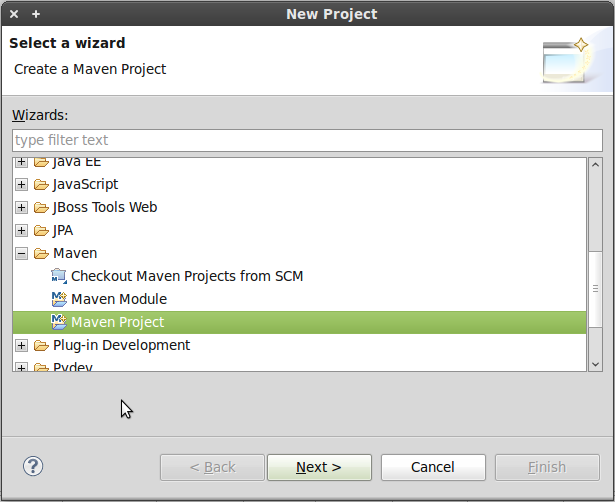
\includegraphics[width=\textwidth]{img/ht01.png}
\caption{Create a new Maven Project.}
\label{fig:maven-project01}
\end{figure}
\begin{figure}
\centering
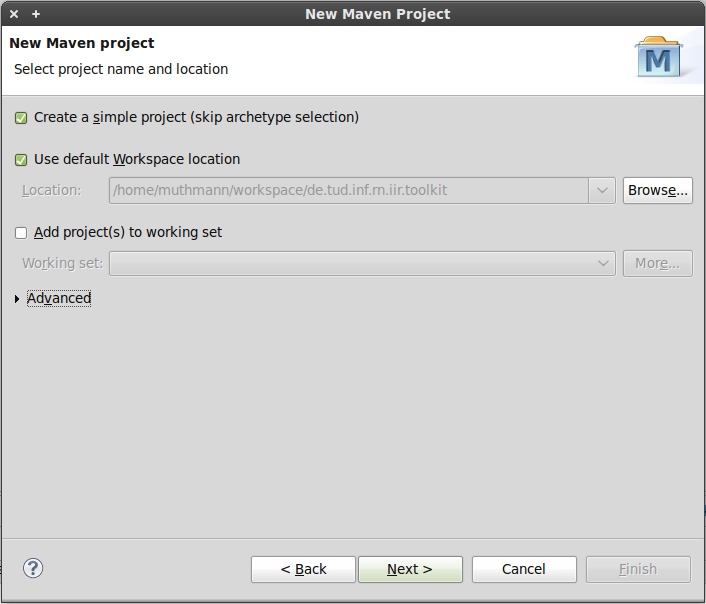
\includegraphics[width=\textwidth]{img/ht02.png}
\caption{Choose to create a simple Maven Project.}
\label{fig:maven-project02}
\end{figure}
\begin{figure}
\centering
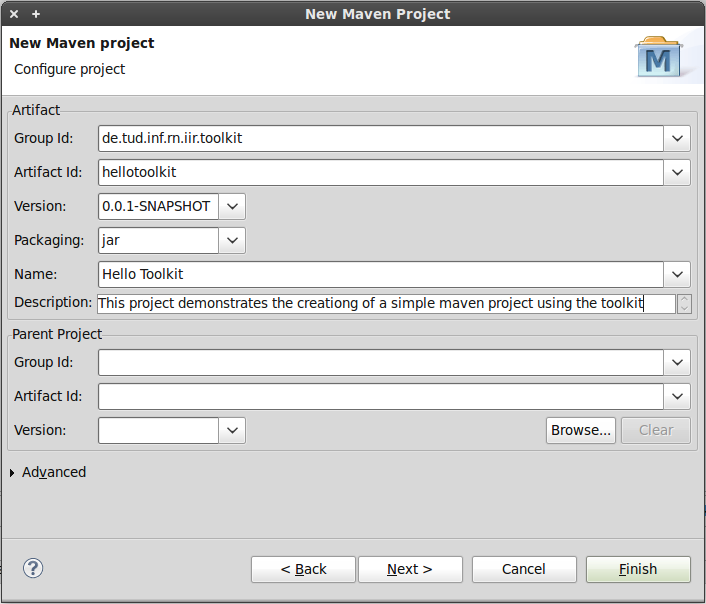
\includegraphics[width=\textwidth]{img/ht03.png}
\caption{Enter detail information about your new Maven Project}
\label{fig:maven-project03}
\end{figure}
\paragraph{Adding the toolkit dependency to the project:} Right click on the new project. In the context menu that appears choose \textit{Maven $\rightarrow$ Add Dependency} (See Fig.~\ref{fig:example-project-context-menu01} and \ref{fig:example-project-context-menu02}).
\begin{figure}
\centering
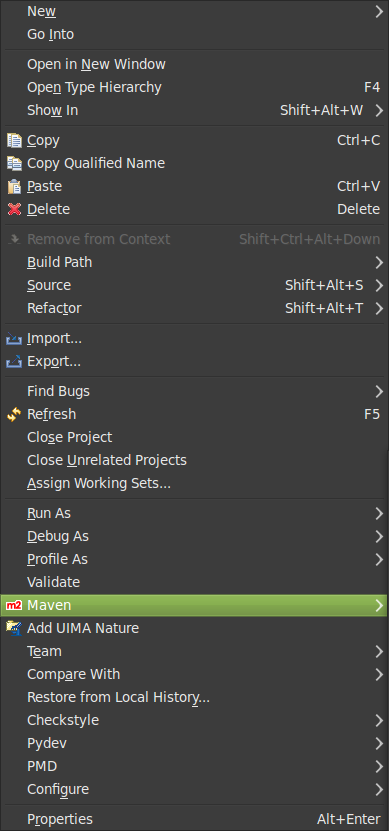
\includegraphics[scale=1]{img/context02.png}
\caption{Maven Project Context Menu. Choose \textit{Maven}}
\label{fig:example-project-context-menu01}
\end{figure}
\begin{figure}
\centering
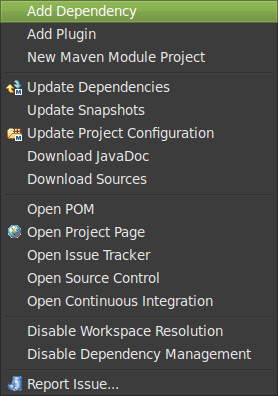
\includegraphics[scale=1]{img/context01.png}
\caption{Create a new Maven project}
\label{fig:example-project-context-menu02}
\end{figure}
A search interface appears (See~\ref{fig:add-dependency01}). If you followed the steps in Section~\ref{sec:buildingthetoolkitusingapachemaven} and installed the toolkit to your local Maven repository, you can type \textit{toolkit} in the search interface (See Fig.~\ref{fig:add-dependency02} and add the dependency with a double click on the \textit{de.tud.inf.rn.iir toolkit} entry. 

Note: If you need to add further dependencies in the future you can use the same steps.
\begin{figure}
\centering
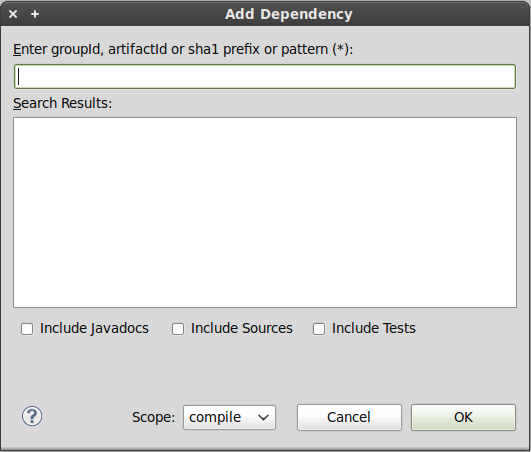
\includegraphics[width=\textwidth]{img/ht04.png}
\caption{Search interface for Maven dependencies.}
\label{fig:add-dependency01}
\end{figure}
\begin{figure}
\centering
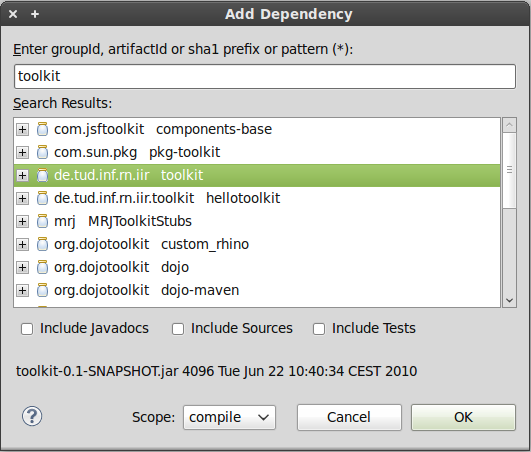
\includegraphics[width=\textwidth]{img/ht05.png}
\caption{Search results for \textit{toolkit}}
\label{fig:add-dependency02}
\end{figure}
The Maven plugin adds the dependency to your pom.xml file, which should look like Fig.~\ref{fig:pom01}.
\begin{figure}
\centering
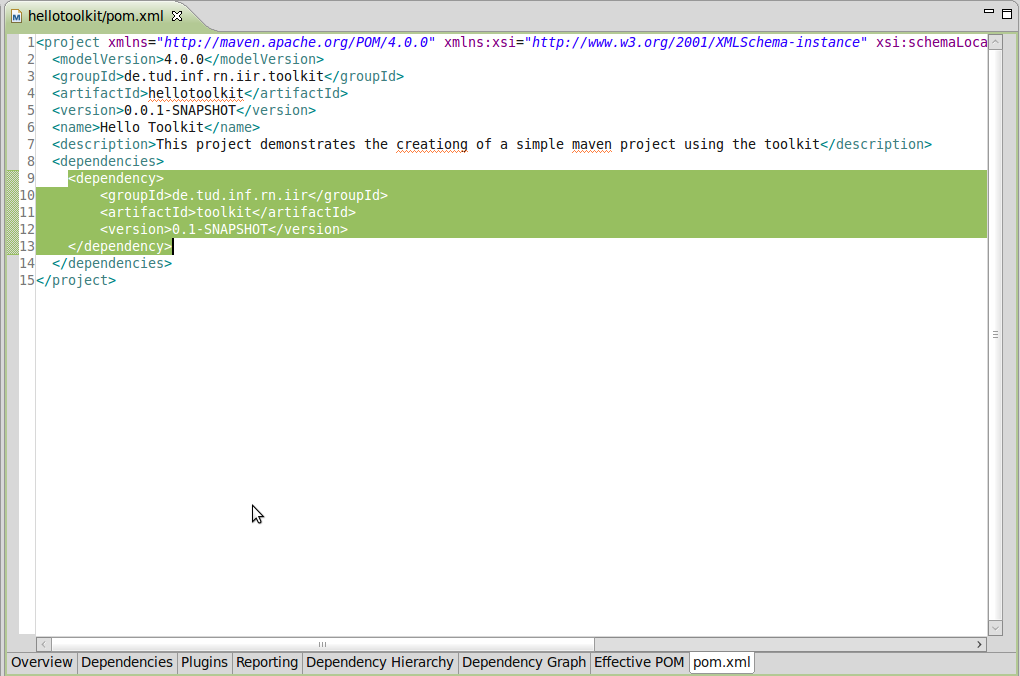
\includegraphics[width=\textwidth]{img/ht06.png}
\caption{POM with added dependency on the TUD Palladian toolkit.}
\label{fig:pom01}
\end{figure}
\paragraph{Configuring your project} Since Maven by default still uses Java 1.4 (conservative), but the toolkit depends on Java 1.6 (current) you need to configure the Maven Java compiler plugin to use Java 1.6 by adding the following markup to your pom.xml (add it after the description element):
\begin{verbatim}
<build>
 <plugins>
  <plugin>
   <groupId>org.apache.maven.plugins</groupId>
   <artifactId>maven-compiler-plugin</artifactId>
   <version>2.3.1</version>
   <configuration>
    <compilerArgument>-Xlint:all</compilerArgument>
    <showWarnings>true</showWarnings>
    <source>1.6</source>
    <target>1.6</target>
    <compilerArguments>
     <encoding>UTF-8</encoding>
    </compilerArguments>
    <showDeprecation>true</showDeprecation>
    <verbose>true</verbose>
    <encoding>UTF-8</encoding>
   </configuration>
  </plugin>
 </plugins>
</build>
\end{verbatim}
It is also necessary to tell Eclipse to use Java 1.6 instead of 1.4. To do this open the project properties via the context menu and choose \textit{Java Compiler} there change all three entries to 1.6. This is shown in Fig.~\ref{fig:java602} and Fig.~\ref{fig:java603}. The project's encoding needs to be set to UTF-8 which can be adjusted in the \textit{Resource} section as shown in Fig.~\ref{fig:utf8}. These properties can also be set for your whole workspace via Eclipse preferences.
\begin{figure}
\centering
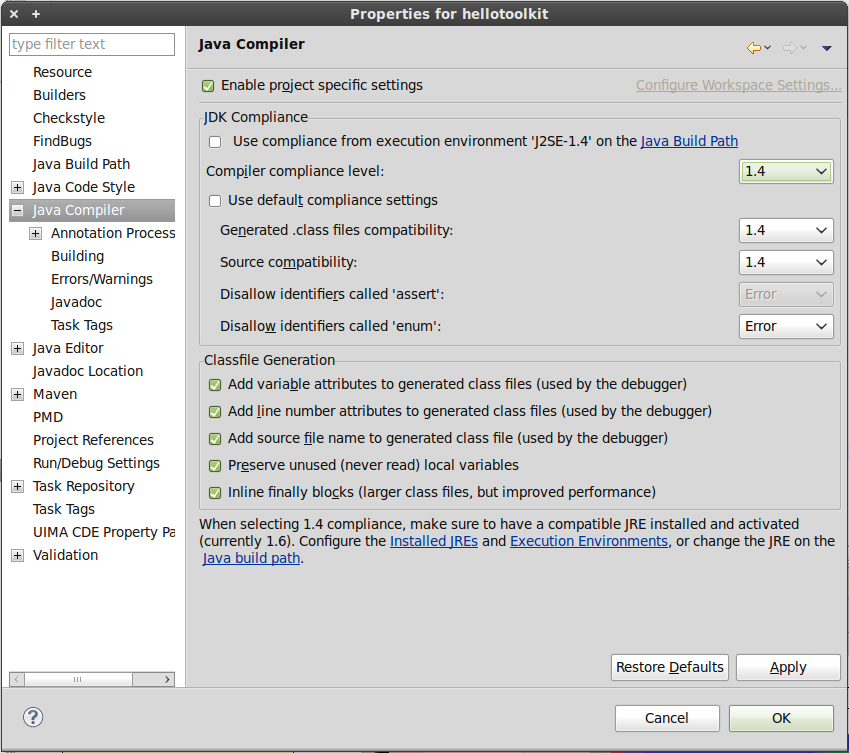
\includegraphics[width=\textwidth]{img/ht08.png}
\caption{Eclipse uses Java 1.4 by default for Maven projects}
\label{fig:java602}
\end{figure}
\begin{figure}
\centering
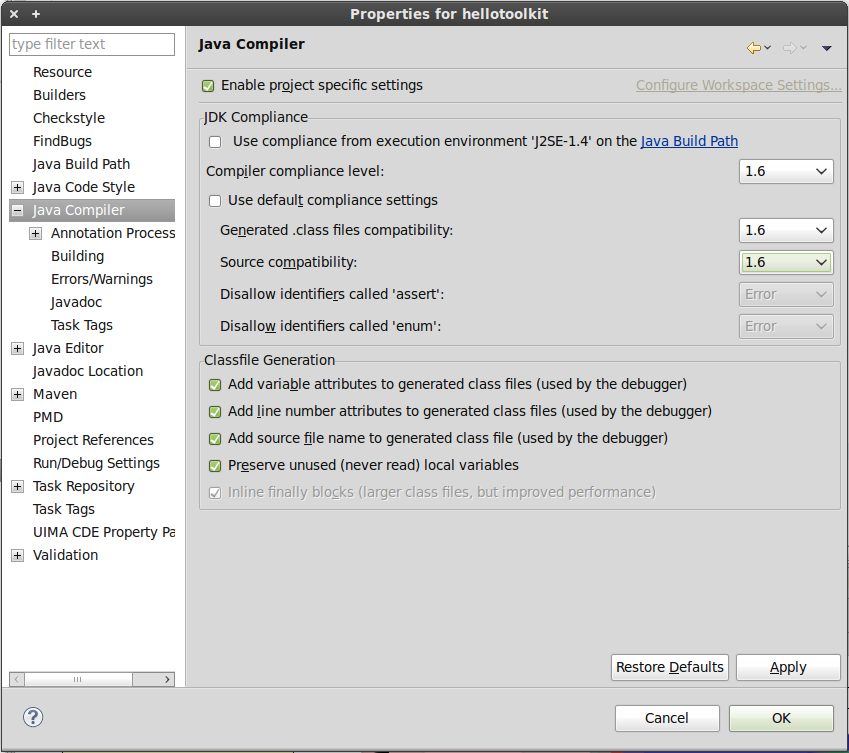
\includegraphics[width=\textwidth]{img/ht09.png}
\caption{Configure Eclipse to use Java 1.6}
\label{fig:java603}
\end{figure}
\begin{figure}
\centering
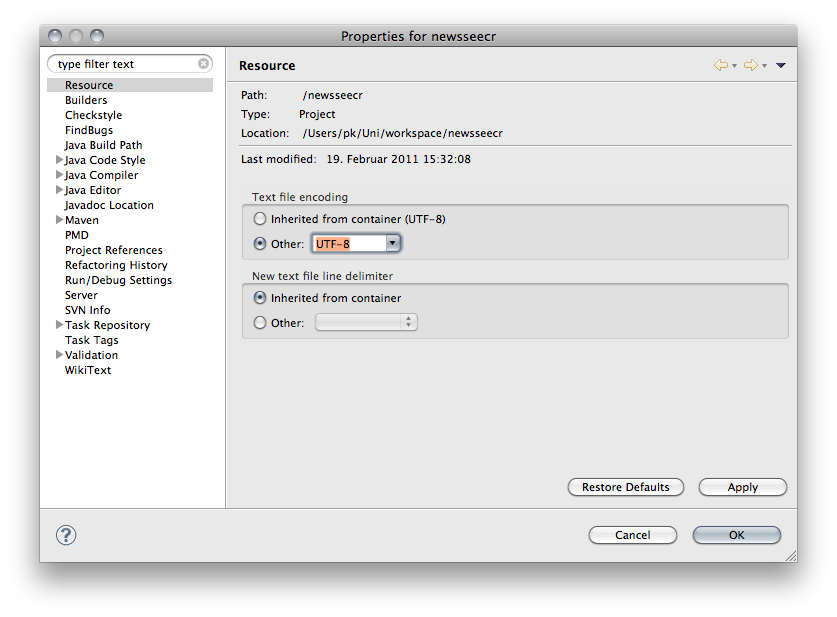
\includegraphics[width=\textwidth]{img/ht16.png}
\caption{Configure Eclipse for UTF-8 encoding}
\label{fig:utf8}
\end{figure}
\paragraph{Writing your first Code with Palladian} Now you can start to write your first code. Your project will already contain the default Maven directory structure. Do not change this structure since Maven depends on it\footnote{Of course you can change Mavens behaviour via the pom.xml but this requires additional configuration not covered by this document. Refer to the Maven documentation under \url{http://maven.apache.org/} for further information.}. As usual we will start with a very simple "Hello World" application. Create a new package \texttt{de.tud.inf.rn.iir.toolkit} and a new class \texttt{HelloToolkit} containing a \texttt{main} method. In this main method you can add actual toolkit code. We used the first example as described in Section~\ref{sec:howto} and search Bing for a string term . The example is also shown in Fig.~\ref{fig:hellotoolkit}.
\begin{figure}
\centering
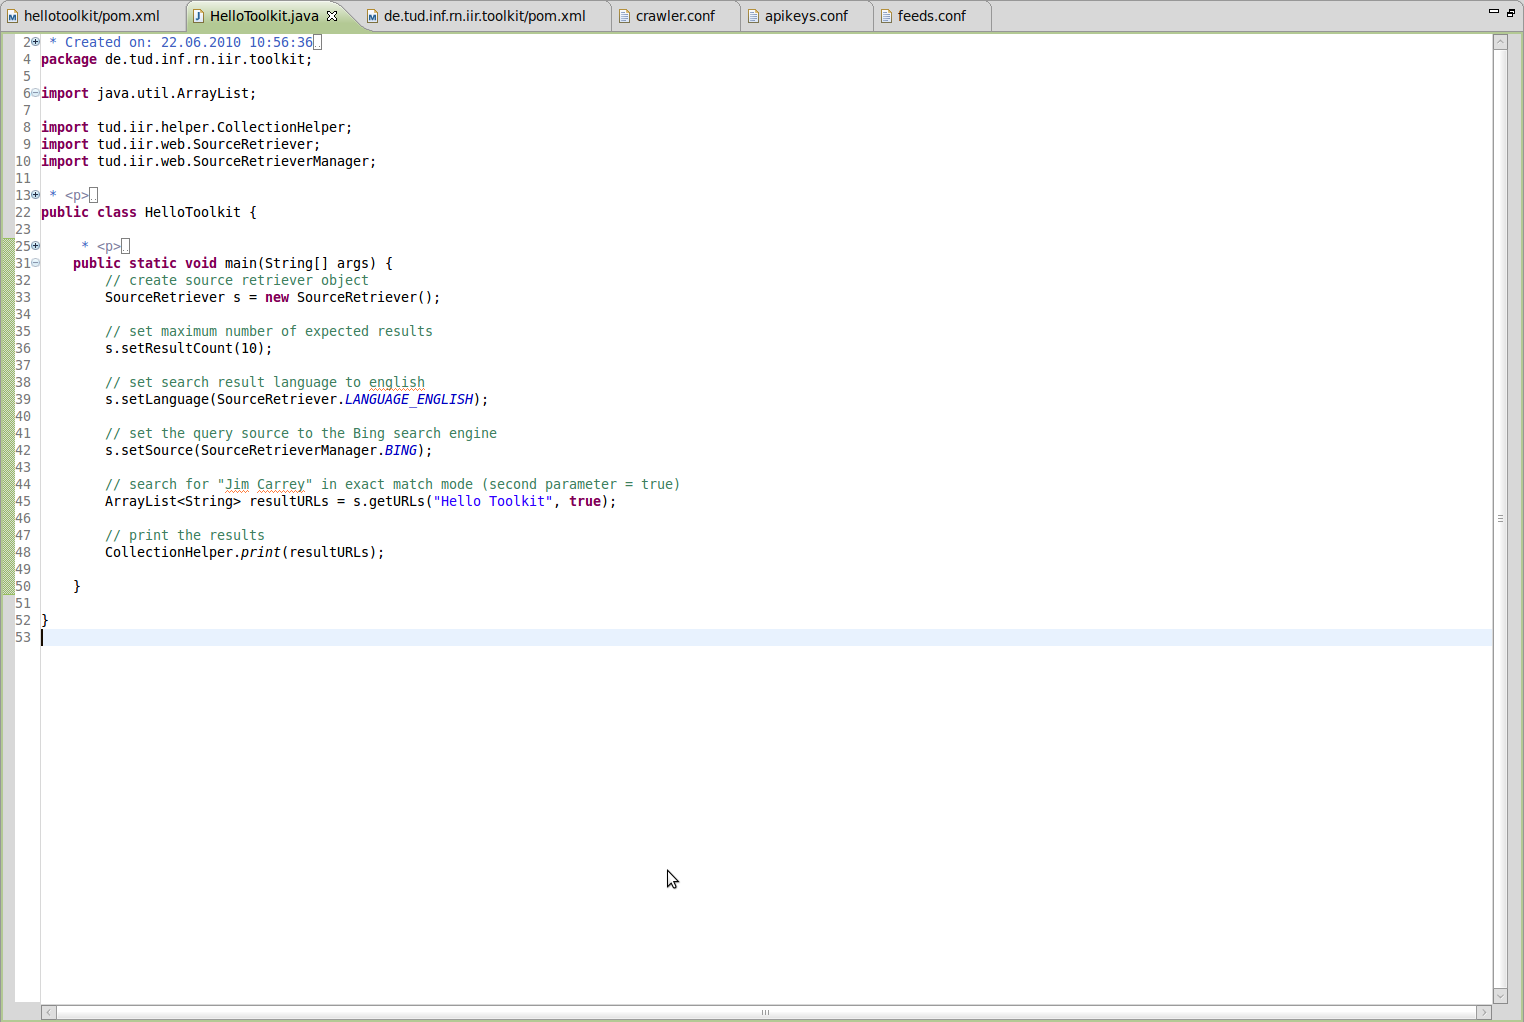
\includegraphics[trim=0 350px 600px 0,clip=true,width=\textwidth]{img/ht10.png}
\caption{"Hello Palladian" Code}
\label{fig:hellotoolkit}
\end{figure}
For the code to work you need copy three files from the config folder in the toolkit project to the config in the source code. These are \texttt{crawler.conf}, \texttt{apikeys.conf} and \texttt{feeds.conf}. You need to copy them to \texttt{src/main/resources/config}. The folder \texttt{src/main/resources} usually contains all resources that are not Java files but are required by your code. All files are shown in Fig.~\ref{fig:resource01}, \ref{fig:resource02} and \ref{fig:resource03}. Fig.~\ref{fig:structure} shows the final directory and file structure of your project.

\begin{figure}
\centering
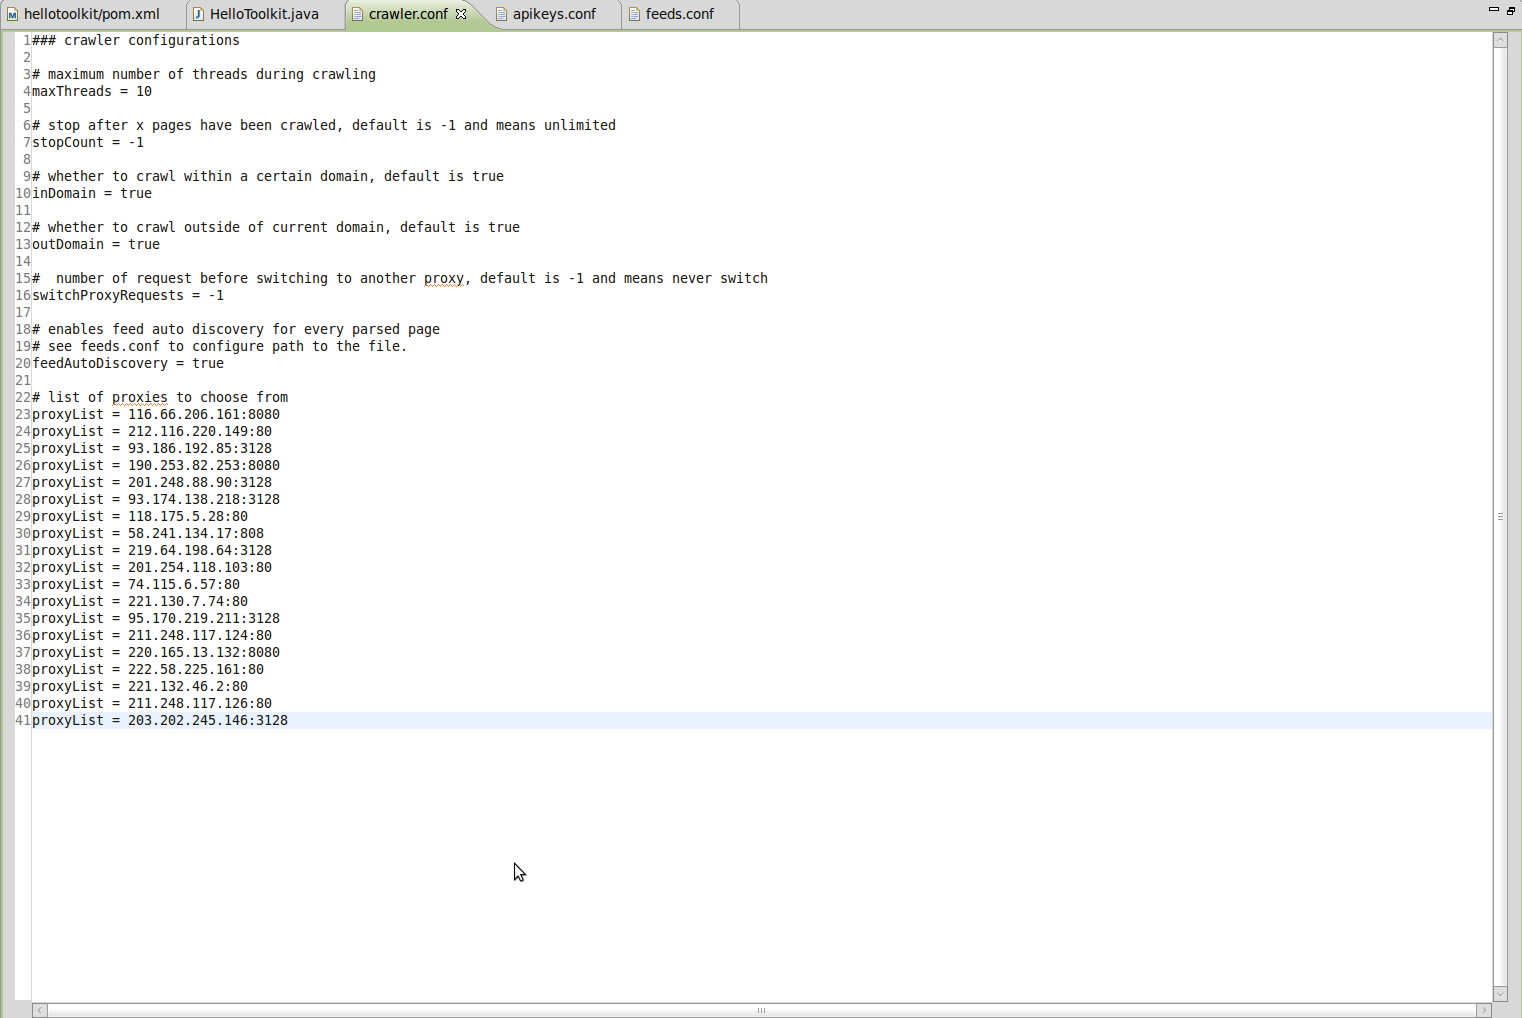
\includegraphics[trim=0 250px 600px 0,clip=true,width=\textwidth]{img/ht11.png}
\caption{\texttt{config/crawler.conf}}
\label{fig:resource01}
\end{figure}
\begin{figure}
\centering
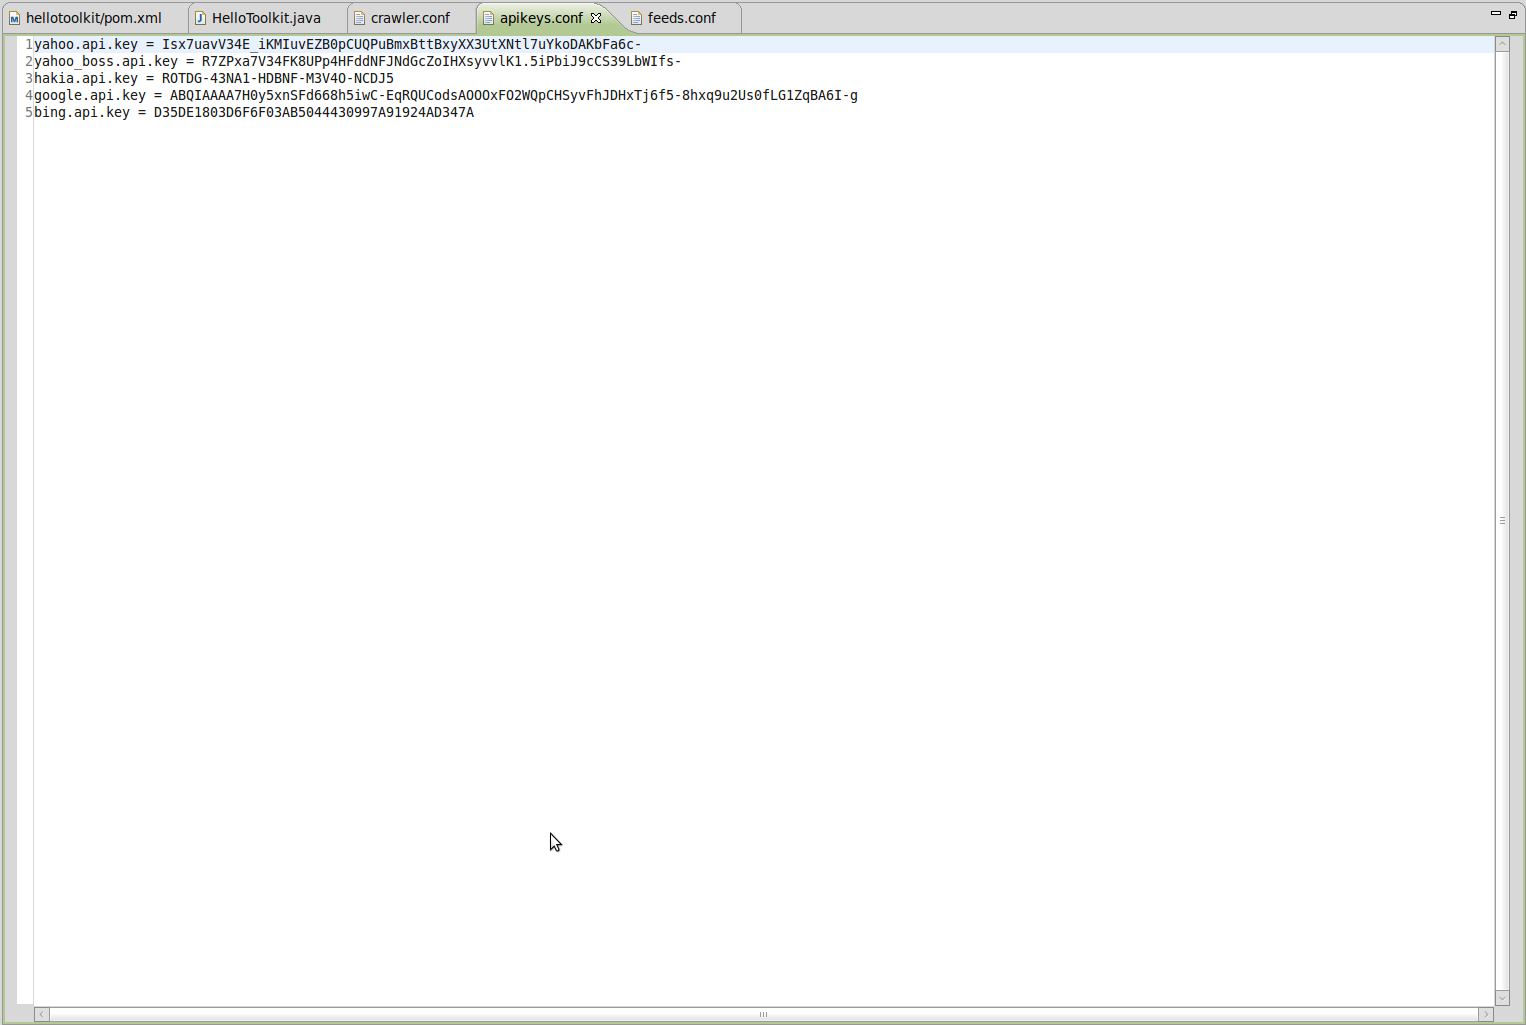
\includegraphics[trim=0 850px 600px 0,clip=true,width=\textwidth]{img/ht12.png}
\caption{\texttt{config/apikeys.conf}}
\label{fig:resource02}
\end{figure}
\begin{figure}
\centering
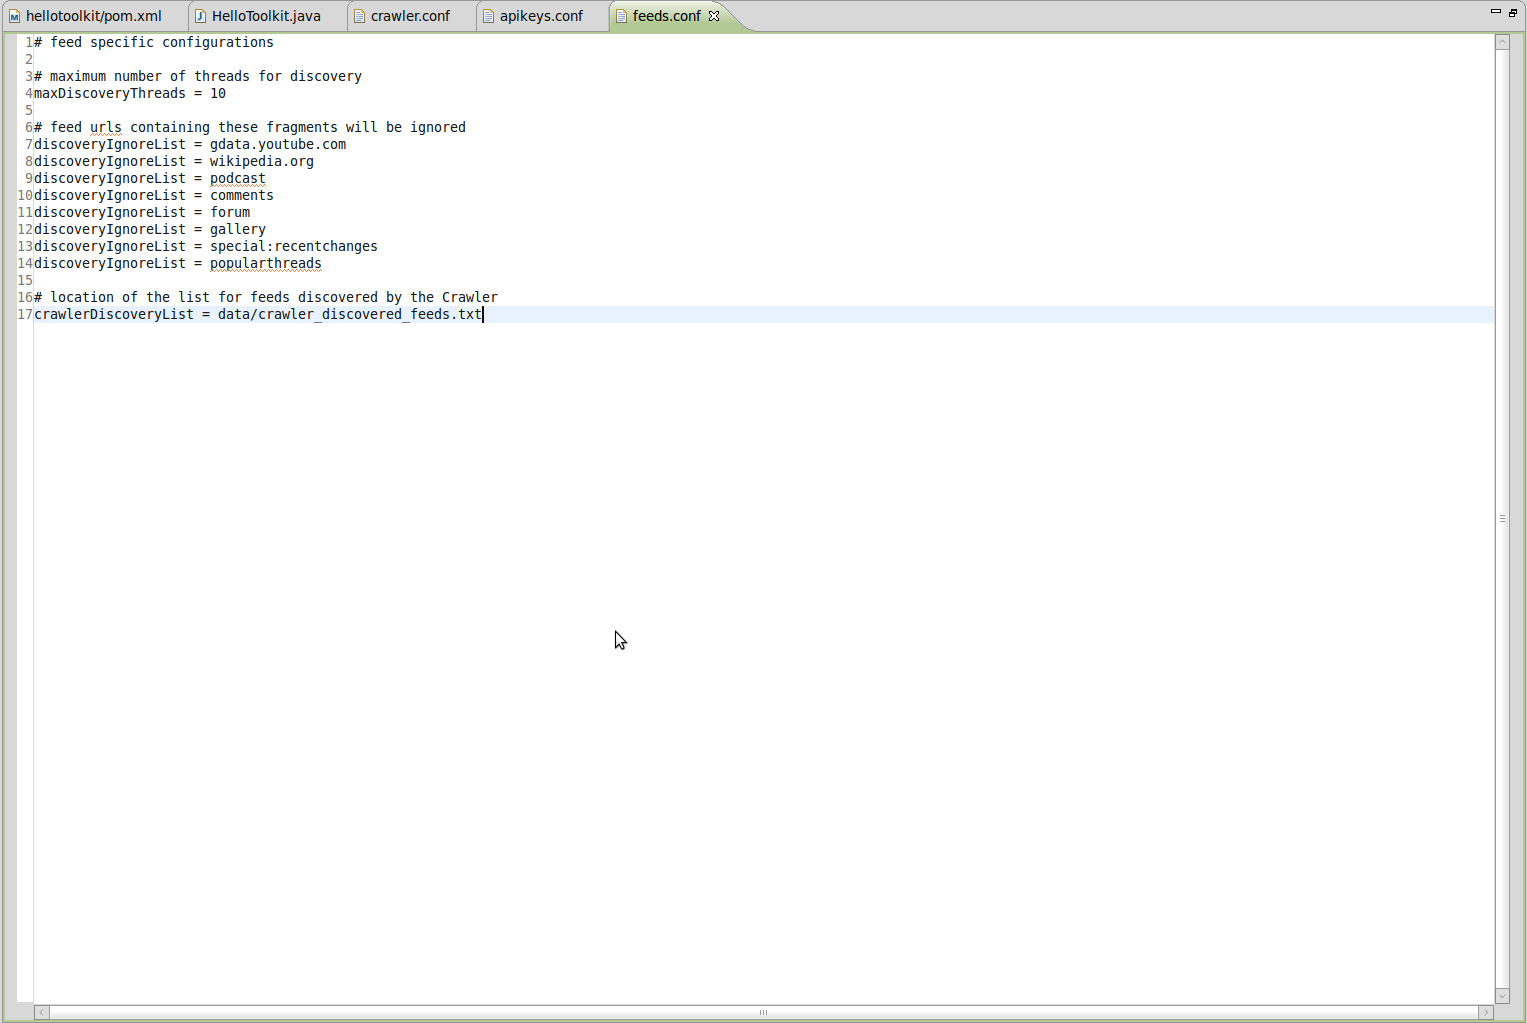
\includegraphics[trim=0 650px 600px 0,clip=true,width=\textwidth]{img/ht13.png}
\caption{\texttt{config/feeds.conf}}
\label{fig:resource03}
\end{figure}
\begin{figure}
\centering
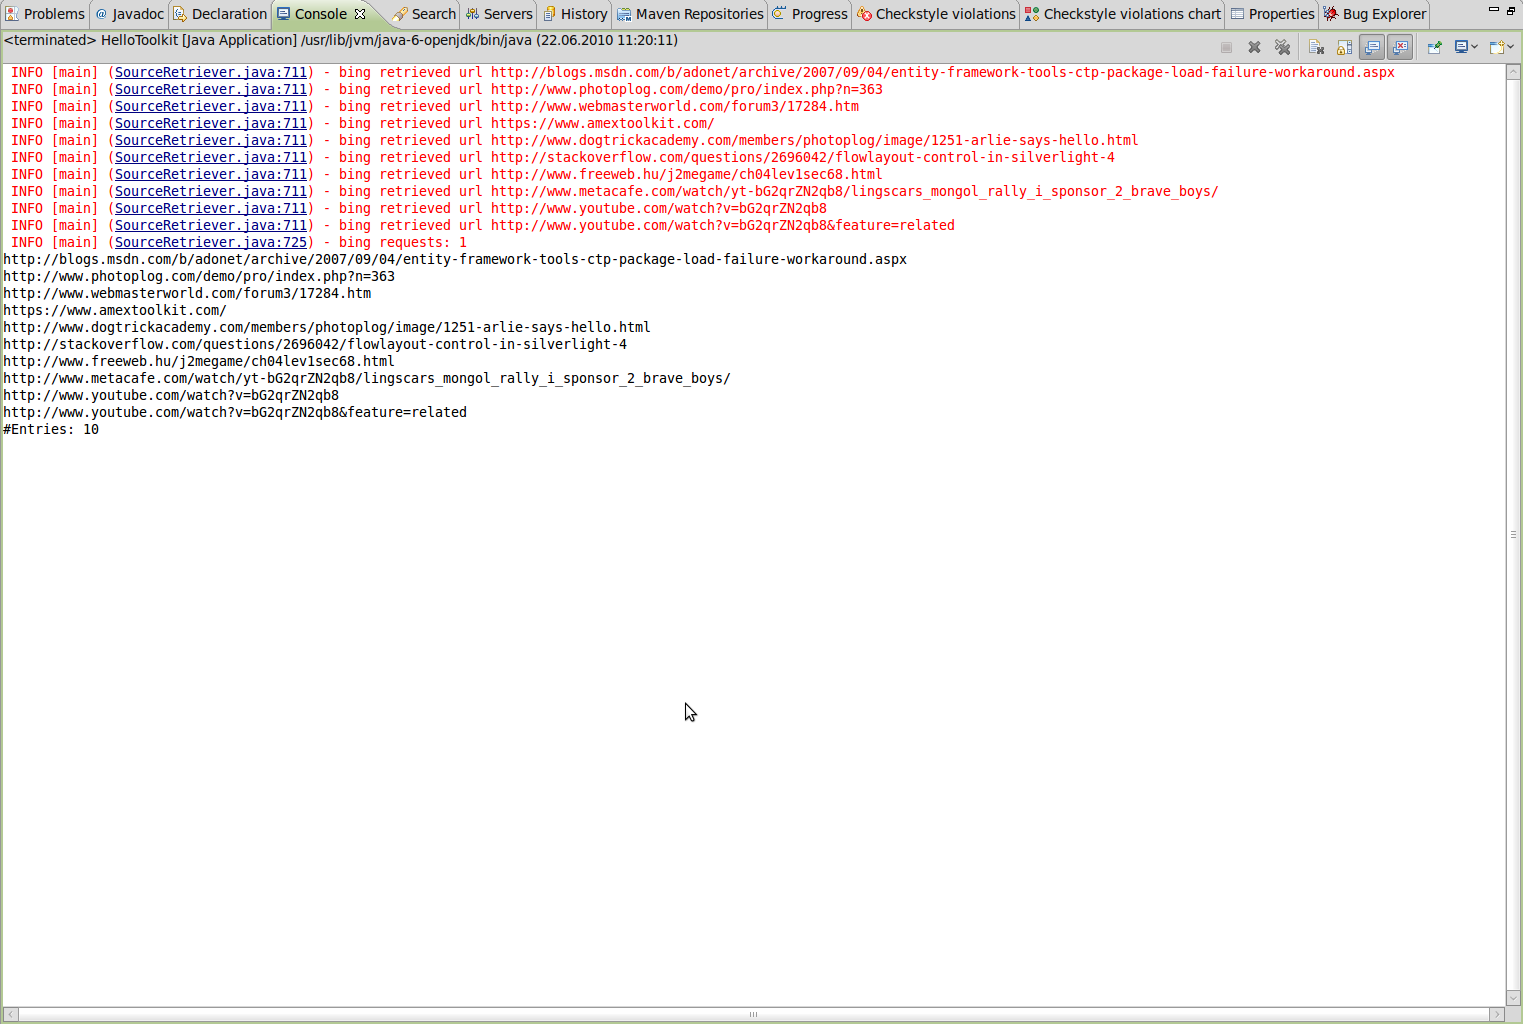
\includegraphics[trim=0 550px 100px 0,clip=true,width=\textwidth]{img/ht14.png}
\caption{"Hello Palladian" Console Output}
\label{fig:structure}
\end{figure}
With the structure from Fig.~\ref{fig:structure} you can run your project. Just open your projects context menu again, choose \textit{Run As $\rightarrow$ Maven Clean}, then open context menu again choose \textit{Run As $\rightarrow$ Maven Install} and finally choose \textit{Run As $\rightarrow$ Java Application}.

\section{Access to Models and Data Sets} \label{sec:AccessModelsDataSets}

Since models and data sets might be very large in file size, they are not included in the SVN repository. As generally no version control is neccessary for this data, we maintain our repository with rsync\footnote{\url{http://rsync.samba.org/}}. rsync is a utility which allows efficient file and directory synchronization between two, local or remote, locations. It was originally developed for Unix systems and should be included with all current Linux distributions and Mac OS X. Altough there are several ports for Windows systems, we recommend using the cwrsync\footnote{\url{http://www.itefix.no/i2/node/10650}} package. 

Palladian comes with convenient ready-to-use scripts to download models and data sets from our central repository. The scripts are called \texttt{dataSync.bat} for Windows and \texttt{dataSync.sh} for Linux and Mac OS X and can be found in the \texttt{dev} directory. Make sure to set the \texttt{DESTINATION} variable inside the script before initial usage. On Windows operating systems, you further need to add the directory with the rsync binaries to your \texttt{PATH} environment variable, which can be done using the ``System Properties'' control panel (See Fig.~\ref{fig:rSyncWindowsPath1} and ~\ref{fig:rSyncWindowsPath2}).

Please contact the toolkit managers if you need write access to the rsync repository.


\begin{figure}
\centering
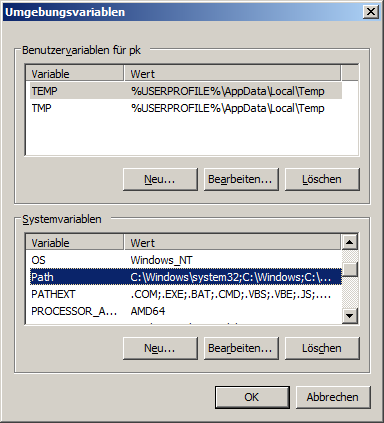
\includegraphics[scale=0.8]{img/WindowsPath1.png}
\caption{Configuring PATH on Windows}
\label{fig:rSyncWindowsPath1}
\end{figure}

\begin{figure}
\centering
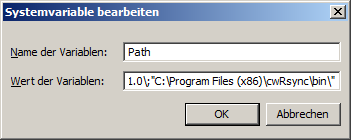
\includegraphics[scale=0.8]{img/WindowsPath2.png}
\caption{Configuring PATH on Windows}
\label{fig:rSyncWindowsPath2}
\end{figure}


\section{Reporting Issues using Redmine}
To report issues with the toolkit or to view issues assigned to you, you need to register to \emph{Redmine}. To do this send an E-Mail to the administrator at \href{mailto:klemens.muthmann@tu-dresden.de}{klemens.muthmann@tu-dresden.de} and provide your name, your advisor, and the reason why you are working on Palladian (i.e. thesis topic or research fellow). You will receive an E-Mail (not automatically so it might take some time) providing a link where you can set your password. If you successfully set a password for your account you can login on: \href{http://redmine.effingo.de/}{Redmine}.

\subsection{Using Redmine directly from Eclipse}
To view \emph{Redmine} tasks directly within \emph{Eclipse} you can use the \emph{Redmine} integration for \emph{\href{http://www.eclipse.org/mylyn/}{Mylyn}}. \emph{Mylyn} is the task tracker plugin of \emph{Eclipse}. It provides connections to most of the popular task and issue tracking systems such as \emph{Trac}, \emph{Bugzilla}, \emph{Jira}, \emph{Mantis}, etc. Unfortunately there is no native support for \emph{Redmine}. Luckily you can add it by installing the \emph{Redmine Connector} plugin using the Update Site \url{http://redmin-mylyncon.sourceforge.net/update-site/N/}. 

After installing the plugin open the \textit{Task Repositories} view and \textit{Add Task Repository}! There should be an entry for \emph{Redmine}. Select it and click \textit{Next \textgreater}! Enter the connection to the Palladian Redmine instance \url{http://redmine.effingo.de} and your credentials or your API key. The API key appears on the right pane in your user settings while logged into \emph{Redmine}. Now \textit{Validate Settings}! \emph{Mylyn} checks the connection to \emph{Redmine}. If successful click \textit{Next \textgreater} and enter a query on which tasks you are going to view inside \emph{Mylyn} on the next page. Click \emph{Finish} and open the \textit{Task List} view to see, edit and create tasks from \emph{Redmine} directly inside \emph{Eclipse}.